\section{前言}
\courseTime{Sep. 6, 2022\\Week 1}先简单介绍一下这门课的总体情况。


2019 年,为辅助申报强基计划,化学系筹划开设一些拔高课程。2020 年第一次开课,对选课学生有要求。这门课是「高阶荣誉课程」,有一定难度。

(\emph{省略历年分数分布})

到了大学之后,每个人的价值取向、人生追求是不一样的。这门课是为了以后硕士阶段的科研准备的,并且紧扣研究生的课程。并不是说你以前成绩不好,就不推荐学习这门课。如果你对物化、物质内部的基本原理感兴趣,我也非常期待你有好成绩。

这门课是有徐昕老师和张颖老师主讲,徐老师比较忙,张老师会先上一部分课,请同学们多担待。我们有两位助教同学:李亚静、范文斌(\url{wbfan21@m.fudan.edu.cn})。关于课堂内容和作业,有不懂的地方,可咨询助教同学。

我们的课程基于量子力学,掰开揉碎了讲。主要有以下几本参考书:
\begin{enumerate}
    \item  Levine, Ira N. \emph{Quantum Chemistry}. Boston: Pearson, 2014. 
    \item  徐光宪,黎乐民,王德民. 量子化学:基本原理和从头计算法 第2版 [M]. 北京:科学出版社, 2021. 
    \item  Atkins P. W and R. S Friedman. \emph{Molecular Quantum Mechanics.} 4th ed. Oxford University Press 2005.
\end{enumerate}

我们的课以板书为主,辅以幻灯片讲解。徐老师上了很多年的课,全部用的板书,我们延续这个传统。如果有任何地方看不清、看不懂,请随时打断我。板书的好处是,所有公式的呈现都是易于理解的,希望能达到对所有公式都「知其然,知其所以然」的程度。

我们还会有一些上机联系,操作 Gaussian 软件。我们学过物化 A I,知道微观世界遵循量子力学原理。化学上感兴趣的绝大多数体系,用薛定谔方程可得到所有的性质,部分含有重原子的体系,需要求解 Dirac 方程。如果只关心基态、定态信息,定态薛定谔方程就足够了。哪怕是定态薛定谔方程,大于两个电子的体系都无法精确求解,所以要用到一些近似方法,如 Hartree--Fock、耦合簇、DFT 等。对我们来说,学习了近似方法之后,要练习如何使用它们。我们以一个水分子为例,水分子的基态能量是多少?氢氧键的键能、键长是多少?等到上机时都可以一试。

稍微有点尴尬的是,从量化的这门课本身来说,其实一学期是不够的。我们学完 18 周,只能讲一些最基础的知识,甚至连最基本近似方法都还讲不到。以至于这门课的后面的上机练习,原则上匹配的是本课程的后续内容。但依然要通过上机对理论计算有个基本的认识。

知识储备要有\boldtext{大学物理}、\boldtext{线性代数}、物理化学 A I。想要能够更深理解,要对线性代数有一些了解。

\chapter{量子力学的诞生}

学完物化之后,对量子力学的印象是什么?

宏观世界与微观电子的运动行为完全是不同的,量子力学革了牛顿力学的命。我们不是在树下乘凉,而是站在巨人的肩膀上。

量子力学中有一些颠扑不破的真理,我们要先信它、认为它是对的,才能用它。为什么这句话的逻辑很重要。本课的本质是量子力学的应用,我们并不探讨量子力学正确与否,先假设它是完全正确的,那么它在化学中的应用是怎样的。

从完整性角度,我们稍微的浏览一遍量子力学的基础,包括量子力学的诞生,我们会从不同的角度去看这个问题。具体的公式不再推导,但是会讲它们的原理、背后的物理概念、思想上的突破、对构建量子力学的帮助。

可能有的同学还是不太相信量子力学,先来回顾一些量子力学里的基本知识。

量子力学中最大的特性是?

\section{波粒二象性}

一个微观粒子,不仅有宏观粒子的属性,也有波的属性。宏观世界中的粒子,可以比作刚性小球,波动性则比作声波,二者用完全不同的方法描述。

粒子用位置和动量描述。波是在整个实空间内离域的,没有局域状态,用频率和振幅描述。

经典物理里,二者是二元对立的。1900 年后的实验表明,二元对立并不能解释实验现象,说明量子力学是从光的思考中得到的。同学们之前都学过,所以这里讲几个重要事件,帮助同学们理清逻辑。

\subsection{黑体辐射}
黑体辐射是指,处于热力学平衡态的黑体发出的电磁辐射的过程。它的重要性来自工业,任何物体的温度与其辐射出的电磁波都有关系,所以可以用颜色来观测冶金过程中金属的温度。特别重要的是,没有黑体辐射的精确解,就不会有发达的武器锻造。太阳光和太阳温度的关系,宇宙微波背景辐射……黑体辐射是物理学中非常基础的现象。

维恩(Wilhelm Wien, 1864---1928)拿了诺贝尔奖(1911 年),他提出的公式在短波相符。瑞丽从统计力学出发,得到了另一个公式,该公式在长波相符较好,在短波爆炸。当时的人们并不认为这里会有新的物理。

1900 年,Planck 从数学模拟出发,讲积分变为求和,让求和的量有固定的间隔,于是得到了量子化的假设,
\begin{equation}
    \varepsilon = h \nu,
\end{equation}
其中 $h$ 是普适的常数——Planck 常量($h = \SI{6.63E-34}{\joule\second}$)。
Planck 的解释是,能量必须是一份份的。换句话说,光在吸收和发射时的能量是一份份的,这与人们早期认为的连续能量是相违背的。但这并不代表光有粒子行为。

\extraInfo{研究范式}{
能量量子化,并不是从原理推导或者是哲学思考。Planck 本人并不相信量子化。

科学有几种范式,第一种是从实验试错,第二种是从理论推导理论推导是说,先建立公理,得到一些规则并去解释实验。二者是相辅相成的,往往是实验总结得到规律,形成定理后反过来再指导实验,这在 2000 年以前是很常见的。

对于化学中的复杂体系,我们看到结果才能解释,比如是氢键或者是立体位阻等。如果我们拿到一个反应,不去做实验是得不到反应机理的,这正是给了理论化学发展的空间。

1950 年计算机发展后,计算科学迅速发展。这是一种新的范式,使用理论去定量模拟复杂体系。理论计算给实验科学赋能,成为了指导实验的重要工具和手段。

在信息爆炸的数据时代,数据就是生产力。大数据是说人们无法掌控的信息量。现在机器学习、人工智能的发展,它有能力从海量的数据中抽取特征,给出新奇的公式和物理图景。大数据可以映射出一些人工永远无法算出来的规则。
元素周期表相当于所有物质的「原子基」,得到了广泛的验证。大数据被认为是未来非常重要的一个研究方式。

物理并不是什么都能做,不同尺度的现象有不同的规则。微观世界由量子力学控制,再多一些粒子就要用统计物理描述。
}

\subsection{光电效应}

黑体辐射是说,光在吸收和发射时是一份份的能量。光电效应则证明了,能量在传播时也是一份份的。爱因斯坦解释了光电效应,获得了 1921 年诺贝尔奖。

背后的物理是,光打到金属表面,如果每一份能量都被完美吸收,只有当 $h\nu_0=A$ 时才会逸出电子。当入射光频率小于临界频率 $\nu < \nu_0$ 时,不能逸出电子,不管能量多大都不能逸出,光子能量以热量耗散掉。当 $\nu > \nu_0$ 时,动能
\begin{equation}
    \frac12mv^2 = h\nu - A = h(\nu - \nu_0). 
\end{equation}

\subsection{固体比热}

爱因斯坦在 1907 年发现,当温度 $T \rightarrow 0\,\mathrm{K}$ 时,固体比热趋于 0。这是一个非常重要的观察。

1910s,很多实验都指向了一个结论,即光是量子化的。

\begin{figure}\centering
\begin{tikzpicture}
    \draw[->, thick] (-5,0) -- (5,0);
    \filldraw[black] (-4,0) circle (2pt) node[below, align=center]{17 世纪\\牛顿:微粒说};
    \filldraw[black] (0,0) circle (2pt) node[below, align=center]{19 世纪前期\\Yang 光的干涉 \\ Maxwell 电磁波};
    \filldraw[black] (4,0) circle (2pt) node[below, align=center]{20 世纪\\光量子理论\\光电效应、黑体辐射};
\end{tikzpicture}
\caption{波粒二象性的认识}
\end{figure}

人们逐渐接受了光的波粒二象性。20 世纪,波动说占主导地位,所有的解释都是从波的表象说起。光如果是波,必然有频率和振幅。光如果是粒子,必然有质量 $m_0$ 和速度 $v$。动量和能量最大的区别是矢量和标量。如何定义光的动量?Planck--Einstein 关系式
\begin{equation}
    E = h\nu. 
\end{equation}
光子以光速运动,不符合牛顿力学,其质量与速度有关,
\begin{equation}
    m = \frac{m_0}{\sqrt{1 - \left(\frac vc\right)^2}}.
\end{equation}
已知
\begin{equation}
    \left\{
        \begin{aligned}
        &E = mc^2 = \frac{m_0c^2}{\sqrt{1 - \left(\frac vc\right)^2}}, \\
        &E = (pc)^2 + (m_0c^2)^2, 
        \end{aligned}
    \right.
\end{equation}
得到
\begin{equation}
    E = pc.
\end{equation}
又因为 $c = \nu\lambda$,有 $cp = h\nu$,即
\begin{equation}
    p = \frac{h\nu}c = \frac h\lambda,
\end{equation}

\subsection{Compton 散射实验}
前面讲的是能量的吸收和发射。粒子有个很重要的行为,即碰撞。1923 年,康普顿证明了碰撞中光的能量和动量是守恒的。

我非常建议大家回去看看这些实验的介绍,因为它非常巧妙,因为要证明这个其实并不容易。他为什么要用 X 射线来设计,反映出来的什么样的实验数据、什么样的物理现象?如果大家经常做实验,我觉得这话题也是很相像的。我们任何的实验的设计,无非是想要得到我们想要证明的某一种化学规则跟物理规定。

于是我们便得到了光的「波粒二象性」结论。我们很难理解光是粒子,同时质量又为零。实际上,光子在运动时具有粒子性,因为碰撞行为跟粒子很相近,运动轨迹也是例子,同时动量也是守恒的。另一方面波动性,因为光子之间有干涉。我们不得不承认波粒二象性。

更具有变革的思维方式是,有质量的物体会有波动性吗?

\subsection{原子结构的确定}
经典力学包含牛顿力学和 Maxwell 波动力学,解释不了电子绕核运动时并不会坍缩。对原子稳定性的解释,引来了经典力学的灾难。为了解决原子稳定性,Bohr 提出\boldtext{量子论},将电子量子化
\begin{equation}
    E_n - E_m = h\nu. 
\end{equation}
光子的能量与能级相匹配,才可以发生跃迁,实验上看到的量子化现象是分立的光谱。证明了 (1) 原子具有能量不连续的性质,(2) 两个定态之间的量子跃迁。

到这里,光有波粒二象性、质量不为零的粒子也有能量量子化的倾向。人们思考,物质是否也有波动性?德布罗意(de Broglie)设想实物粒子也可以有粒子与波的两重性,即物质波(matter wave),
\begin{equation}
    \left\{
        \begin{aligned}
            &E = h\nu,\\
            &\lambda = \frac hp, 
        \end{aligned}
    \right.
    \rightarrow
     \nu = \frac Eh. 
\end{equation}

不管当时的历史争论,\textbf{微观粒子的运动需要一种全新的力学规则}。如果微观粒子既有波动性,也有粒子性,那么它一定不遵循牛顿力学。波意味着全空间分散,粒子意味着局域的、有因果关系的,这两个是完全不一样的概念。从原子结构的确定、物质波的提出,意味着微观粒子需要不同的力学规则。

1926 年,建立薛定谔方程,表示微观粒子的波动方程。

一个理论之所以完美,是因为在它的深部潜藏着某种真实的东西。爱因斯坦对玻尔理论说的话「这是思维领域中最优美的音乐」,可能他想说,伪学说无法和谐。\footnote{〔苏〕达宁, 华燕. 概率世界 [M]. 沈阳:辽宁科学技术出版社, 1985. 118. }

\subsection{电子衍射}

1927 年,Davison、Gramer 发现了电子衍射现象。

至此,量子完成了所有预备,开始了飞速发展。

\begin{figure}\centering
    \begin{tikzpicture}
        \node[above] at (-2,0) {Bohr 量子论};
        \draw[->] (-2,0) -- (-2,-0.5);
        \node[below] at (-2,-0.5) {W. Heisenberg 矩阵力学};
        \node[above] at (3,0) {de Broglie 物质波};
        \draw[->] (3,0) -- (3,-0.5);
        \node[below, align=center] at (3,-0.5) {Schrodinger 波动力学\\(量子化学中常用)};
    \end{tikzpicture}
    \caption{量子力学的两种诠释}
\end{figure}

我们回顾了量子力学的起源,所以本章取名「波粒二象性」。微观粒子最大的特性就是波粒二象性,所有的物理现象,所有的思维上的冲突、革命,都基于人们对于一个粒子能否具有波动性、一个波能否具有粒子性,这样一个冲突争论、思考、妥协,最后形成规律,所有的事情现象都是这样。物质科学的本质还是实验,不断去解释实验。人们厉害的地方就是,通过实验总结出来的规律可形成定义,定义时不可以证明的,唯一的用处是证明实验是对的。从逻辑角度来说,定义就是一个更高层级的规则,具有普适性。

物理学背后的发展哲学是「Less is beautiful.」「小就是美」。牛顿力学的本质是质点轨迹,统计物理的本质是等概率,几何光学的本质是费马原理,这些都无法证伪。从物理角度来说,所有理论都有一个核心,可以延伸出所有其它理论。一旦偏执于这种思维,当碰到某些东西可能非常困难。

在现在的机器学习时代,如果某天物理、数学可以由机器主动获取,你是觉得 dirty 还是 beautiful?这就是历史的洪流,不可阻挡。

\homework{
    \textbf{1.1} 重温黑体辐射的历史,论述 Wein 与 Rayleigh--Jeans 公式的内在异同。论述 Planck 如何利用「能量量子化」的概念,从 Rayleigh--Jeans 公式中得到 Planck 黑体辐射公式。
}

希望同学们知道,物理定律从来都不是证明的。从逻辑上来说,它们是逻辑的起点,是基于实验现象的总结,是普适的、完备的。NASA 得到的宇宙微波辐射与 Planck 的公式完全符合,说明宇宙本身是讲规矩的。从温度极高的太阳,到黑洞、宇宙大爆炸后残余的微波辐射,都满足量子化的公式,这是很有趣的。

我们知道了微观粒子不遵循牛顿力学、遵循薛定谔方程,那么如何推导薛定谔方程?新的物理概念一定是从原有的物理大厦中借鉴来的,比如描述波动的薛定谔方程,一定是从 Maxwell 方程中得到了启发,进而构建了这个研究方向,并用原子的精细光谱证明了这个方向是对的。这个过程不是推导,是演绎、启发、相互佐证,有复杂的逻辑。

下面,从波的角度,演绎波动方程跟薛定谔方程、跟 Maxwell 方程有什么异同点,怎么导出能量算符、动量算符。很多内容没法证明,只能说服自己它就是它。
下节课,我们会从波动方程,推导出薛定谔方程,演绎出算符。本质上并不意味着这些内容可以推导,同学们要把这些定理和公式当成公理般的存在,这些公理的基础是来自实验的能量量子化结论。

\section{一维单色平面波}
\courseTime{Sep. 5, 2022\\Week 1}
我们回顾了量子力学的发展的这个过程,重要的是波粒二象性的发现。当大家从无数的实验中间承认了波粒二象性之后,大家已经接受了微观跟宏观世界是不一样的,微观粒子并不遵循牛顿力学,因果率不一样。既是波又是粒子,意味着微观粒子既离域又定域。那么很多时候,宏观能够唯一决定的状态,在微观就不能够决定了,经典运动轨迹就不会有了。

现在的问题就是,我知道它是不一样的,那到底遵循什么样的一个运动方程呢?建立运动方程过程,不可能是从石头里面蹦出来,我们不可能无中生有、凭空造出来。但是,我们又知道,物理的定律是没法什么推导,也没法证伪。意味着,在物理定律的构造过程中,一定闪耀的是人类最宝贵的创造力。创造力怎么来?一定是基于我们对物质世界的一个观察、总结、升华,而且肯定有很多的借鉴、对比。最终抽提、精炼、凝结成的几条定律,并可以在实验中被反复验证。

通过跟波动方程的一个关联,去探讨是质量不为零的物质到底遵循什么样的波动方程,它跟 Maxwell 方程里面的波动方程到底有什么相同、不同?这不是证明,只是对比。

\subsection{推导表达式}
Maxwell 方程中的一维单色平面波满足的波动方程是
\begin{equation}
    \label{eq:mono_wave}
    \frac{\partial^2 \psi(x,t)}{\partial x^2} = \frac{1}{c^2} \frac{\partial^2 \psi(x,t)}{\partial t^2},
\end{equation}
它有两项,对位置的二阶偏导、对时间的二阶编导。

任何数学物理方程,在实际情况中的应用,一定离不开\boldtext{边界条件}的确定。没有边界条件是没有办法解数据物理方程的。对于一般的单色波,(1) 有空间的\boldtext{周期性},任意移动一个波长后相等,(2) 沿时间任意传播一定频率后相等,
\begin{align}
    &\psi(0,t) = \psi(\lambda, t), \label{eq:mono_wave_periodical}\\
    &\psi(x,0) = \psi\left(x,\tfrac\lambda{c}\right) \label{eq:mono_wave_freq}
\end{align}
接下来求解方程 \eqref{eq:mono_wave}。这个方程非常典型的特点就是,坐标的偏导放一边,时间偏导放一边,不出现坐标和时间的耦合 $\frac{\partial}{\partial x}\frac{\partial}{\partial t}$。这就意味着,坐标波函数与时间波函数可以\boldtext{分离变量}。不失一般性地,令波函数 $\psi (x,t) = \phi(x) f(t)$,代回方程 \eqref{eq:mono_wave} 有
\begin{equation}
    f(t) \frac{\partial^2 \phi(x)}{\partial x^2} = \frac{\phi(x)}{c^2} \frac{\partial^2 f(t)}{\partial t^2},
\end{equation}
两边同除 $\phi(x) f(t)$,有
\begin{equation}
    \frac1{\phi(x)} \frac{\partial^2 \phi(x)}{\partial x^2} = \frac{1}{c^2 f(t)} \frac{\partial^2 f(t)}{\partial t^2},
\end{equation}
现在就有问题了,什么时候两边可以同除?换种说法,具备什么品质的波函数可以同除?在某些物理条件下,波函数可以为 0,并不一定是可以除的。这个在后面讲到量子力学基本假设的时候会讲到。

\extraInfo{精确解}{
任何可以分离变量的体系都可以精确解,面试时经常问道这个问题。数学上来讲,不能分离变量成单变量的函数不可以精确解。

一维势箱可以精确求解,三维势阱分离 $xyz$ 变量后也可以精确求解。氢原子原则上是不能精确求解的,其原子核和电子有耦合。如果在 Born--Oppenheimer 近似下,固定原子核不动,将原子核当成参数,电子的运动可以在极坐标下严格拆分成径向和角度部分,超过 2 个电子依然不能精确求解。

只要能分离变量,哪怕势函数是复杂的,就可以精确求解。氢分子 \ce{H2} 不能精确求解,两个电子之间有耦合 $\frac1{r_{12}}$。氢分子离子 \ce{H2+} 只有一个电子是可以精确求解的,这里电子受到的是椭球势,该体系在 1950s 是非常热门的话题,可以解得 $\pi, \sigma$ 等轨道。
}

分离变量后,得到
\begin{equation}
    \left\{
        \begin{aligned}
            &\frac1{\phi(x)} \frac{\partial^2\phi(x)}{\partial x^2} = K, \\
            &\frac1{c^2f(t)} \frac{\partial^2 f(t)}{\partial t^2} = K,
        \end{aligned}
    \right.
\end{equation}
将上式化为微分方程的标准型,得到坐标和时间分量的二阶微分方程,
\begin{numcases}{}
    \frac{\partial^2\phi(x)}{\partial x^2} - K \phi(x) = 0, & \label{eq:mono_wave_phi}\\
    \frac{\partial^2 f(t)}{\partial t^2} - K c^2f(t) = 0, & \label{eq:mono_wave_time}
\end{numcases}
下面分别讨论这两个单变量方程。对 \eqref{eq:mono_wave_phi},有通解
\begin{equation}
    \phi(x) = A \exp(a x),\label{eq:mono_wave_phi_general}
\end{equation}
将通解代回 \eqref{eq:mono_wave_phi} 有
\begin{equation}
    a^2 \exp(ax) = K \exp(a x),
\end{equation}
得到 $a = \pm \sqrt K$,波函数 $\phi(x) = A \exp(\pm \sqrt K x)$。为了满足周期性边界条件 \eqref{eq:mono_wave_periodical},有
\begin{equation}
    \ee^0 = \exp (\pm \sqrt K \lambda) = 1,
\end{equation}
分类讨论 $K$,
\begin{enumerate}
    \item $K > 0$,此时有平凡解 $\lambda = 0$,不考虑,
    \item $K = 0$,$\phi(x) = \text{constant}$,不考虑,
    \item $K < 0$,令 $p = -K >0$,则 $\exp (\pm \ii \sqrt p \lambda) = 1$,得到 $\sqrt p \lambda = 2\pi$,即 $p = \frac{4\pi^2}{\lambda^2}$,$K = -\frac{4\pi^2}{\lambda^2}$。
\end{enumerate}
将解代回通解 \eqref{eq:mono_wave_phi_general},有
\begin{equation}
    \phi(x) = A \exp(\pm \ii \sqrt p x) = A \exp(\pm \ii k x), \quad k = \frac{2\pi}{\lambda}. \label{eq:mono_wave_phi_sol}
\end{equation}
其中 $k$ 称为光的波矢。同理,对于时间变量的微分方程 \eqref{eq:mono_wave_time},仿照坐标分量的求解过程,
设通解
\begin{equation}
    f(t) = B \exp (b t), \label{eq:mono_wave_time_general}
\end{equation}
解得 $b = \pm c\sqrt{K}$。将频率的边条件 \eqref{eq:mono_wave_freq} 代入通解 \eqref{eq:mono_wave_time_general},有
\begin{equation}
    \ee^0 = \exp \left(\pm c \sqrt K \frac\lambda{c}\right) = 1,
\end{equation}
分类讨论可知 $ k \geqslant 0$ 应舍去,当 $k<0$ 时,设 $q = -k>0$,则 $\exp(\pm \sqrt K \lambda) = \exp(\pm \ii\sqrt q \lambda) = 0$,得到 $\sqrt q \lambda = 2\pi$,即 $b = \pm \ii c \frac{2\pi}\lambda$。将解代回通解 \eqref{eq:mono_wave_time_general} 有
\begin{equation}
    f(t) = B \exp\left(\pm\ii \,\omega t\right) = B \exp \left(\pm \ii \,c \frac{2\pi}\lambda t\right),\quad \omega = \frac{2\pi c}{\lambda} = 2\pi \nu,
\end{equation}
其中 $\omega$ 是角频率。

最终,我们求解出了单色波的波动方程,
\begin{equation}
    \psi(x,t) = \phi(x) f(t) = C \exp[-\ii(k x \pm \omega t)]. \label{eq:mono_wave_sol}
\end{equation}
注意到,其中的 $\omega$ 和 $k$ 有\boldtext{线性关系} $\omega = k c$。

% 讨论传播方向
定义约化 Planck 常量 $\hbar = \frac{h}{2\pi}$,又成为 Dirac 常量,类似角频率的定义。于是有
\begin{equation}
    E = h\nu = \hbar \, 2\pi \nu = \hbar \omega. 
\end{equation}
\subsection{传播方向}
波动方程 \eqref{eq:mono_wave_sol} 中的正负号表示什么意思?

我们知道,复空间上的指数可以用欧拉方程表示成三角函数,有
\begin{equation}
    \phi(x,t) = C_1 \cos (k x\pm \omega t)-\ii C_2 \sin (k x \pm \omega t),
\end{equation}
\begin{lstlisting}
ExpToTrig[C Exp[-I (k x + \[Omega] t)]]
>> C Cos[k x + t \[Omega]] - I C Sin[k x + t \[Omega]]
\end{lstlisting}
在实数域 $\mathbb{R}$ 上,波动方程为
\begin{equation}
    \phi(x,t)|_\mathbb{R} = C \cos(k x\pm \omega x),
\end{equation}
当 $kx\pm\omega t=2\pi n, n \in \mathbb{Z}$ 时,波动方程处于节点,观察这些节点的移动方式。

当 $t = 0$,$x = \frac{2\pi n}{k}$,当 $t = t_1$ 时,有
\begin{equation}
    x = \frac{2\pi n \mp \omega t_1}k = \frac{2\pi n}k \mp \frac{\omega t_1}k,
\end{equation}
这一点的速度即为
\begin{eqnarray}
    v = \frac{\partial x}{\partial t} = \mp\frac{\omega}k = \mp c.
\end{eqnarray}
所以结论是,正号对应左移,负号对应右移。
\begin{figure}\centering
    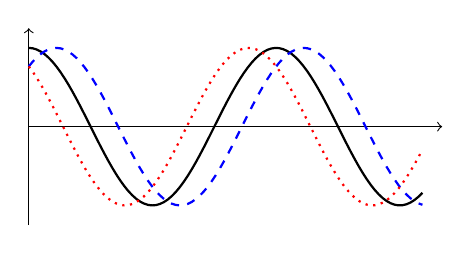
\begin{tikzpicture}[scale=0.5]
        % axis
        \draw[->] (0,0) -- (10.5, 0);
        \draw[->] (0,-2.5) -- (0, 2.5);
        % functions
        \draw[domain=0:10,black,thick,samples=100] plot (\x,{2*cos(deg(\x))});
        \draw[domain=0:10,blue,thick,samples=100,dashed] plot (\x,{2*cos(deg(\x-0.7))});
        \draw[domain=0:10,red,thick,samples=100,dotted] plot (\x,{2*cos(deg(\x+0.7))});
    \end{tikzpicture}
    \caption{实空间内波动方程的运动方向,虚线表示右移,点线表示左移}
\end{figure}

我们从一维单色光的平面波出发,可以第一性地给出波函数 \eqref{eq:mono_wave_sol},其中 $C$ 是光强。实空间部分是完全离域的,它是一个球谐函数,可以从 $-\infty$ 到 $+\infty$ 的震荡,其中时间的部分表示传播的方向。这种离域性用来描述光的波动性没问题,但是无法描述粒子性,有无定域的波也满足波动方程?

\section{光波的波包}
动力学中常用\boldtext{波包}描述具有粒子行为的光波。定义
\begin{equation}
    \label{eq:wp_def} % wave packet definition
    \psi(x,t) = \int_{- \infty}^{+ \infty} A(k) \exp \big[ \ii \big( k x - \omega(k) t \big) \big] \, \mathrm{d} k,
\end{equation}
与单色光不同的是,其中放开了两个变量作为波数的函数——振幅 $A(k)$ 与频率 $\omega(k)$。对于单色光,给定了 $k$ 就确定了 $\omega$ 和波函数,所以一个 $k$ 就相当于一个单色光。对每一个的单色光的某种振幅分布的全空间积分,即为一种光的组合,称之为波包。为何称为「包」,后面从图像上解释。

于是 $A(k)$ 是光强振幅,描述波包的形状,$\omega(k)$ 是频率,描述波包的移动速度。

这个波包是否满足波动方程 \eqref{eq:mono_wave}?证明之。分别对坐标和时间求偏导,有
\begin{align*}
    \frac{\partial^2\psi(x,t)}{x^2} 
    &= \int_{-\infty}^{+\infty} A(k) \frac{\partial \ee^{\ii kx}}{\partial x^2} \exp(-\ii\,\omega(k) t) \,\dd k \\ 
    &= \int_{-\infty}^{+\infty} A(k) (-k^2) \frac{\partial \ee^{\ii kx}}{\partial x^2} \exp[\ii(kx - \omega(k)t)] \,\dd k,
\end{align*}
\begin{align*}
    \frac{\partial^2\psi(x,t)}{t^2} 
    &= \int_{-\infty}^{+\infty} A(k) \ee^{\ii kx} \frac{\partial}{\partial t^2}\exp(-\ii\,\omega(k) t) \,\dd k \\ 
    &= \int_{-\infty}^{+\infty} A(k) \left[-\omega(k)\right]^2 \ee^{\ii kx} \exp[\ii(kx - \omega(k)t)] \,\dd k, \\
\end{align*}
观察可知,当 $\omega(k) = ck$ 时,满足波动方程 \eqref{eq:mono_wave}。结论是,单色波的各种分布的组合同样满足波动方程。下面引入一种特殊的波包。

\suppInfo{波包与波动方程}{我们可以说,$\psi(x,t)$ 仍然是光波波动方程的解。这通过将上述 $\psi(x, t)$ 代入波动方程很容易验证。从物理的角度,事实上,如果表达式 $\omega(k) = c k$ 始终成立,那么被积函数 $\exp \big[ \ii \big( k x - \omega(k) t \big) \big]$ 就是波矢为 $k$ 的单色光。由于波动方程的特性,两个不同波矢 (或等价地说波长) 的单色光的线性叠加仍然是波动方程的解,而积分又可以看作是无数不同波长的光波的线性叠加,因此 $\psi(x,t)$ 仅仅就是复色光,它仍然满足单色光所满足的波动方程。

但是这种复色光有很有意思的特性,那就是我们可以通过合适地定义振幅 $A(k)$,使得 $\psi(x,t)$ 具有局域形状,并且该函数可以被归一化。我们应当注意到,单色光的表达式是不可归一化的,宏观上就是在全空间上宽度为常数的波形。}

\subsection{Gaussian 波包}

定义波包的振幅为 Gaussian 型函数,
\begin{equation}
    A(k) = \frac{\sqrt{a}}{(2 \pi)^{3/4}} \exp \left[ - \frac{a^2}{4} (k - k_0)^2 \right]. \label{eq:wp_gaussian_def}
\end{equation}

首先讨论,当 $t = 0$ 的时波包的情况,此时的波函数
\begin{equation}\label{eq:wp_t0}
\psi(x, 0) = \int_{-\infty}^{+\infty} \frac{\sqrt{a}}{(2 \pi)^{3/4}} \exp \left[ - \frac{a^2}{4} (k - k_0)^2 \right] \exp \left( i  k x  \right) \, \dd k. 
\end{equation}
为了求出这个积分,引入傅里叶变换(Fourier transform),
\begin{align}
    &F(x) = \int_{-\infty}^{+\infty} f(k) \ee^{\ii kx}\,\dd k, \\
    &f(k) = \frac1{2\pi}\int_{-\infty}^{+\infty} F(x) \ee^{\ii kx}\, \dd x, 
\end{align}
其中 $f(x)$ 右侧的 $\frac{1}{2\pi}$ 也可拆成两个 $\frac1{\sqrt{2\pi}}$、将其中一个 $\frac1{\sqrt{2\pi}}$ 乘在 $F(x)$ 右边,这是傅里叶变换的多种等价表示方式。傅里叶变换可将时域 $f$ 变换为频域 $F$,相当于一种卷积,这里仅将它用作求积分公式。Gaussian 函数的傅里叶变换为
\begin{align}
    &G(k) = \frac a{\sqrt \pi} \ee^{-a^2 k^2}, \\
    &g(x) = %\frac{1}{\sqrt{2\pi}} 
    \int_{-\infty}^{+\infty} G(k) \ee^{\ii kx} \dd k =  \frac{1}{\sqrt{2\pi}} \exp\left(-\frac{x^2}{4a^2}\right), \label{eq:ift_gaussian}
\end{align}
%{Gaussian 函数的逆变换}
\begin{lstlisting}
res = InverseFourierTransform[a/Sqrt[Pi] Exp[-a^2 k^2], k, x];
Simplify[res, Assumptions -> {a > 0}]
>> E^(-(x^2/(4 a^2)))/Sqrt[2 \[Pi]]
\end{lstlisting}
因此将 $t_0$ 时的波包,拼凑成傅里叶逆变换 \eqref{eq:ift_gaussian} 的形式,有
\begin{equation}
    \psi(x, 0) = \frac{\sqrt{a}}{(2 \pi)^{3/4}}  \ee^{i  k_0 x} \int_{-\infty}^{+\infty} \exp \left[ - \frac{a^2}{4} (k - k_0)^2 + i(k-k_0)x  \right] \dd k,
\end{equation}
设 $b = \frac a2$,$l = k-k_0$,则上式为
\begin{equation}
    \psi(x, 0) = \frac{2b}{(2 \pi)^{3/4}} \ee^{i  k_0 x} \int_{-\infty}^{+\infty} 
    \ee^{-b^2l^2} \ee^{\ii l x} \dd l, 
\end{equation}
凑出 \eqref{eq:ift_gaussian} 中的形式,在积分内乘 $\frac b{\sqrt{\pi}}$,同时令 $x = - 2\pi x'$,
\begin{align}
    \psi(x,0) &= \frac{2b}{(2 \pi)^{3/4}} \ee^{\ii k_0 x} \frac{\sqrt{\pi}}b \underbrace{\int_{-\infty}^{+\infty} \frac b{\sqrt{\pi}} \ee^{-b^2l^2} \ee^{\ii l (-2\pi x')} \dd l}_{\text{inverse Fourier transform}} \\
    &= \frac{2b}{(2 \pi)^{3/4}} \ee^{\ii k_0 x} \frac{\sqrt{\pi}}b  \exp\left(-\frac{\pi^2x'^2}{4 b^2}\right) \\
    &= \left(\frac{2}{a^2\pi}\right)^{1/4} \ee^{\ii k_0 x} \exp\left(-\frac{x^2}{a^2}\right). \label{eq:wp_photon_t0}
\end{align}
\begin{lstlisting}
Integrate[
 Sqrt[a]/(2 Pi)^(3/4)
   Exp[-a^2/4 (k - k0)^2] Exp[I k x], {k, -Infinity, Infinity}, 
 Assumptions -> {a > 0}]
>> (E^(x (I k0 - x/a^2)) (2/\[Pi])^(1/4))/Sqrt[a]
\end{lstlisting}
于是我们推导出了 0 时刻的 Gaussian 波包。%,并且该波包是归一化的,
%TODO: 并不归一吧

当 $t > 0$ 时,有
\begin{equation}
    \psi (x, t) = \left( \frac{2}{\pi a^2} \right)^{1/4} \exp \left[ - \frac{(x - ct)^2}{a^2} \right] \exp [ \ii k_0 (x - ct) ]. 
\end{equation}
\homework{
    \textbf{1.2}  利用傅里叶变换,推导 $t>0$ 的 Gaussian 波包。
}

\begin{figure}\centering
    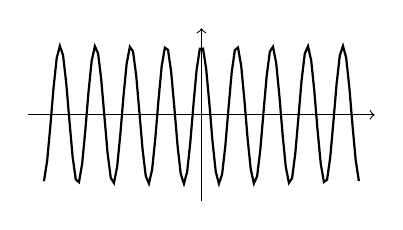
\begin{tikzpicture}[scale=0.5]
        % axis
        \draw[->] (-4.4,0) -- (4.4, 0);
        \draw[->] (0,-2.2) -- (0, 2.2);
        % functions
        \draw[domain=-4:4,black,thick,samples=100] plot (\x,{1.75*cos(deg(7*\x))});
    \end{tikzpicture}
    \begin{tikzpicture}[scale=0.5]
        % axis
        \draw[->,white] (0,-2.2) -- (0, 2.2);
        % functions
        \node[] at (0,0) {$\times$};
    \end{tikzpicture}
    \begin{tikzpicture}[scale=0.5]
        % axis
        \draw[->] (-4.4,0) -- (4.4, 0);
        \draw[->] (0,-2.2) -- (0, 2.2);
        % functions
        \draw[domain=-4:4,black,thick,samples=100] plot (\x,{1.75*exp(-0.25*\x*\x)});
    \end{tikzpicture}
    \begin{tikzpicture}[scale=0.5]
        % axis
        \draw[->,white] (0,-2.2) -- (0, 2.2);
        % functions
        \node[] at (0,0) {$=$};
    \end{tikzpicture}
    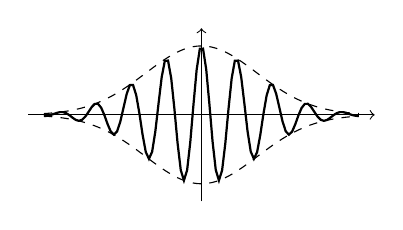
\begin{tikzpicture}[scale=0.5]
        % axis
        \draw[->] (-4.4,0) -- (4.4, 0);
        \draw[->] (0,-2.2) -- (0, 2.2);
        % functions
        \draw[domain=-4:4,black,thick,samples=100] plot (\x,{1.75*exp(-0.25*\x*\x)*cos(deg(7*\x))});
        \draw[domain=-4:4,black,samples=100,dashed] plot (\x,{1.75*exp(-0.25*\x*\x)});
        \draw[domain=-4:4,black,samples=100,dashed] plot (\x,{-1.75*exp(-0.25*\x*\x)});
    \end{tikzpicture}
    \caption{0 时刻波包的组成}
\end{figure}
接下来探讨这个波函数有什么样的性质。一个全空间离域的单色波矢,乘上一个高斯函数,所以形成了这样一个波包。波与波包都是以光速 $c$ 向正方向传播,并且没有任何衰减、变形,最大振幅为 $\left( \frac{2}{\pi a^2} \right)^{1/4}$。

\section{实物粒子的 Gaussian 波包}
德布罗意告诉我们,有静止质量的物体,既是波也是粒子。那么,实物粒子能不能用高斯波包来表示?单色光波的话有个很重要的关系 $\omega = kc$,频率和波矢有直接的关系,但是实物粒子不是这样的。现在我们要将光波波包向实物粒子过渡,以尝试从波动性的角度解释实物粒子。

但这里或许会遇到一个问题,实物粒子不会以 $c$ 的光速传播,因此 $\omega = ck$ 的表达式不成立。我们要如何定义角频率 $\omega$ 与波矢 $k$?

假设现在并不是狭义相对论的,或者说实物粒子以较低速度运动。在经典力学下,自由粒子 (不受外势场 $V (x)$ 影响的粒子) 的能量(即动量)为
\begin{equation}
    E = \frac{p^2}{2m}, \quad \text{for particle}
\end{equation}
考虑波粒二象性,粒子的能量必然也有物质波所对应的能量表述,
\begin{align}
    &E = h\nu = \hbar \omega, \\
    &p = \hbar k, 
\end{align}
上两式同样也适用于无质量的光子。对于实物粒子而言,联立上面的式子消去 $E,p$ 可得
\begin{equation}
    \omega = \frac{\hbar^2k^2}{2m},
\end{equation}
注意到,实物粒子的波矢与角频率是平方的关系,这是与光子最大的区别。

同样使用波包 \eqref{eq:wp_def} 和高斯波包 \eqref{eq:wp_gaussian_def} 的原始定义,得到 $t =0$ 时刻的波函数与光波 \eqref{eq:wp_photon_t0} 是一样的,但 $t > 0$ 的波函数就完全不一样了。

\subsection{精确解}
尽管积分非常复杂,但这仍然是有解析解的。当 $t > 0$ 时,
\begin{equation}
    \psi(x,t) = \left(\frac{2}{\pi a^2}\right)^4 \frac1 {\sqrt{ 1 + \dfrac{2\hbar t}{ma^2}\ii}} \exp \frac {\displaystyle -\frac{x^2}{a^2}-\frac{\ii k_0^2 t \hbar }{2 m}+\ii
    k_0 x} {1 + \dfrac{2\hbar t}{ma^2}\ii},
\end{equation}
所以概率分布为
\begin{equation}
    |\psi(x, t)|^2 = \sqrt{\frac{2}{\pi a^2}} \frac{1}{\sqrt{1 + \displaystyle \frac{4 \hbar^2 t^2}{m^2 a^4}}} \exp \left[ - \frac{2}{a^2} \frac{\left( x - \displaystyle \frac{\hbar k_0}{m} t \right)^2}{1 + \displaystyle \frac{4 \hbar^2 t^2}{m^2 a^4}} \right]. 
\end{equation}

我们应当得到以下的结论:
\begin{itemize}[nosep]
  \item 指前因子可以表示波包的最大振幅。对于光波,其振幅恒定;但对于实物粒子,其振幅会依 $t$ 增长而递减,且递减的程度表现为类双曲线型;
  \item 指数项分母表示波包展宽。对于光波,其展宽恒定;但对于实物粒子,其展宽依 $t$ 增长而递增,且递增的程度表现为类双曲线型;
  \item 指数项分子表示波包的移动速度。对于光波,其移动速度为 $c$,与每个波矢 $k$ 分项的移动速度相同;而实物粒子的移动速度 (波包群速度) 为 $\hbar k_0 / m$,而波矢为 $k_0$ 的单色波对应的移动速度 (相速度) $\omega(k_0) = \hbar k_0 / 2m$,两者相差两倍。
\end{itemize}

这也就意味着,如果用 Gaussian 波包的方式描述自由粒子,即使规定 $t = 0$ 时具有较窄的波包展宽,足够长时间后也总会扩散。“足够长的时间”与物质的质量有关。假设电子的半径大约为 \SI{2.81E-15}{\metre};在一秒时间内仍然处于自由粒子状态。若使用波包解释,那么它现在的半径就在一秒钟内扩大了如下倍数:
\begin{equation}
\sqrt{1 + \frac{4 \hbar^2 t^2}{m_\mathrm{e}^2 r_\mathrm{e}^4}} 
= \sqrt{1 + \frac
{4\times(\num{1.05E-34})^2\times1}
{(\num{9.11E-31})^2(\num{2.82E-15})^4}
}
\simeq \num{2.92E25}
\end{equation}
\begin{lstlisting}
Clear[\[HBar], me, re]
\[HBar] = 1.05457182*10^-34;
me = 9.1093837*10^-31;
re = 2.8179*10^-15;
Sqrt[1 + (4 \[HBar]^2 1)/(me^2 re^4)]
>>2.91586*10^25
\end{lstlisting}
短短一秒,电子似乎会变得比太阳还要大。当然,对于宏观的物体而言,情况就不太一样了。假设一个人在宇宙大爆炸时期诞生,重 \SI{76}{\kilo\gram},想象成为 \SI{1}{\metre} 展宽的波,那么他可能在 2021 年时膨胀了 \num{7.20E-37} 倍。

\iffalse
目前为止,我们还不能说实物粒子波包的物理模型是错误的 (事实上,实物粒子波包模型确实是 Schr\"odinger 方程的解)。只有当物质质量足够大、初始时刻展宽足够宽时,波包能重现经典物理的图像。但想要通过波来刻画粒子的行为,似乎会在微观世界变得不太直观。我们会说这是朴素的波粒二象性的理解,它仍然是试图将粒子通过波的行为描述,而产生看似谬误的结论。

一种可能的理解是,所谓波性与粒性不应朴素地理解,物质的行为在长时间未观测时是不可知的;而在测量时,若使用检测波形的手段就会使得波函数坍缩到接近平面光波的形式;若使用检测粒子的手段则会使波函数接近 $\delta$ 函数的粒子形貌。这称为波包的收缩;依据一些量子力学表述,这比较接近关于波函数投影的假设。

但这不仅是 Gaussian 波包的困难。事实上,对于任意的 $A(k)$ 即任意波包,当时间足够长,波包总会弥散。这可以通过求取不确定度 $\langle x^2 \rangle - \langle x \rangle^2$ 给出;这需要使用到 Ehrenfest 定理。(Cohen-Tannoudji, LIII, Exercise 4)
\fi

\section{从自由粒子波函数到 Schr\"odinger 方程}

\subsection{非相对论 Schr\"odinger 方程}

Schr\"odinger 方程 \textbf{不可导出} ,它一般会作为量子力学的假定出现 (尽管说从 Dirac-von Neumann 公理体系能导出 Schr\"odinger 方程)。但若我们只考虑自由电子 (即不考虑外加势场),那么 Schr\"odinger 方程某种程度上可以通过波包函数导出。

我们仍然以实物粒子的波包函数出发:
\begin{gather}
  \psi(x, t) = \int_{- \infty}^{+ \infty} A(k) \exp \big[ i \big( k x - \omega(k) t \big) \big] \, \mathrm{d} k \\
  E = \hbar \omega \quad p = \hbar k \\
  E = \frac{p^2}{2 m} \quad \omega = \frac{\hbar k^2}{2 m}
\end{gather}
我们希望找到一个偏微分方程,使得 $\psi(x, t)$ 是该偏微分方程的解。但需要注意到,光波方程是不可行的,譬如 $\exp \big[ i \big( k x - \omega(k) t \big) \big]$ 满足下述方程
\begin{equation}
\frac{\partial^2 \psi}{\partial x^2} = \frac{k^2}{\omega^2} \frac{\partial^2 \psi}{\partial t^2} \quad \mathrm{(failed)}
\end{equation}
之所以这个方程在光波上允许,但粒子上不行,是因为对于光波,$k^2/\omega^2$ 恰好是 $1/c^2$ 为常数,但对于粒子而言则为 $(2m/\hbar k)^2$,并非是常数。上述描述波函数的方程只能用于 $k$ 是唯一值的情况,不能用于包含各种不同的 $k$ 的波包因此不应当使用该方程。

但很容易地会想到,之所以会出现 $\omega^2$ 是因为 $\psi$ 对时间 $t$ 作两次偏导时,其前面的系数 $\omega$ 也就被抽提了两次 (这对于 $k$ 也是类似的)。但如果现在只对 $t$ 作一次偏导,那么就只会抽提一次 $\omega$;并且 $k^2 / \omega$ 是常数 $2m/\hbar$,因此就解决了方程中出现的与 $k$ 有关的项。

沿着这个思路,我们就尝试对 $\psi(x, t)$ 分别作 $x$ 的二阶导、$t$ 的一阶导:
\begin{align}
  \frac{\partial^2 \psi}{\partial x^2} &= - \int_{- \infty}^{+ \infty} k^2 A(k) \exp \big[ i \big( k x - \omega(k) t \big) \big] \, \mathrm{d} k \\
  \frac{\partial \psi}{\partial t} &= - \int_{- \infty}^{+ \infty} \frac{i \hbar k^2}{2 m} A(k) \exp \big[ i \big( k x - \omega(k) t \big) \big] \, \mathrm{d} k
\end{align}
因此,
\begin{equation}
\frac{\partial \psi}{\partial t} = \frac{i \hbar}{2 m} \frac{\partial^2 \psi}{\partial x^2}
\end{equation}
即
\begin{equation}
i \hbar \frac{\partial \psi}{\partial t} = - \frac{\hbar^2}{2 m} \frac{\partial^2 \psi}{\partial x^2}
\end{equation}
这就是自由粒子所满足的 Schr\"odinger 方程。

